\documentclass[pdf, aspectratio=169]{beamer}
\usepackage[]{hyperref, graphicx, siunitx, lmodern, tikz, booktabs}
\usepackage[mode=buildnew]{standalone}
\usepackage{pdfpc-commands}

\usetheme{WU2}
\graphicspath{ {Images/} }

\sisetup{per-mode=symbol}
\usetikzlibrary{calc, patterns, decorations.markings, decorations.pathmorphing, shapes}
\tikzstyle{image}=[inner sep=0pt, outer sep=0pt]

\AtBeginSection[]{
	{
	\setbeamertemplate{footline}{}
	\begin{frame}
		\begin{tikzpicture}[remember picture, overlay]
			\fill[red] (current page.north west) rectangle (current page.south east);
			\node[opacity=0.4, anchor=south east, inner sep=0pt, outer sep=0pt] at ([xshift=2cm]current page.south east) {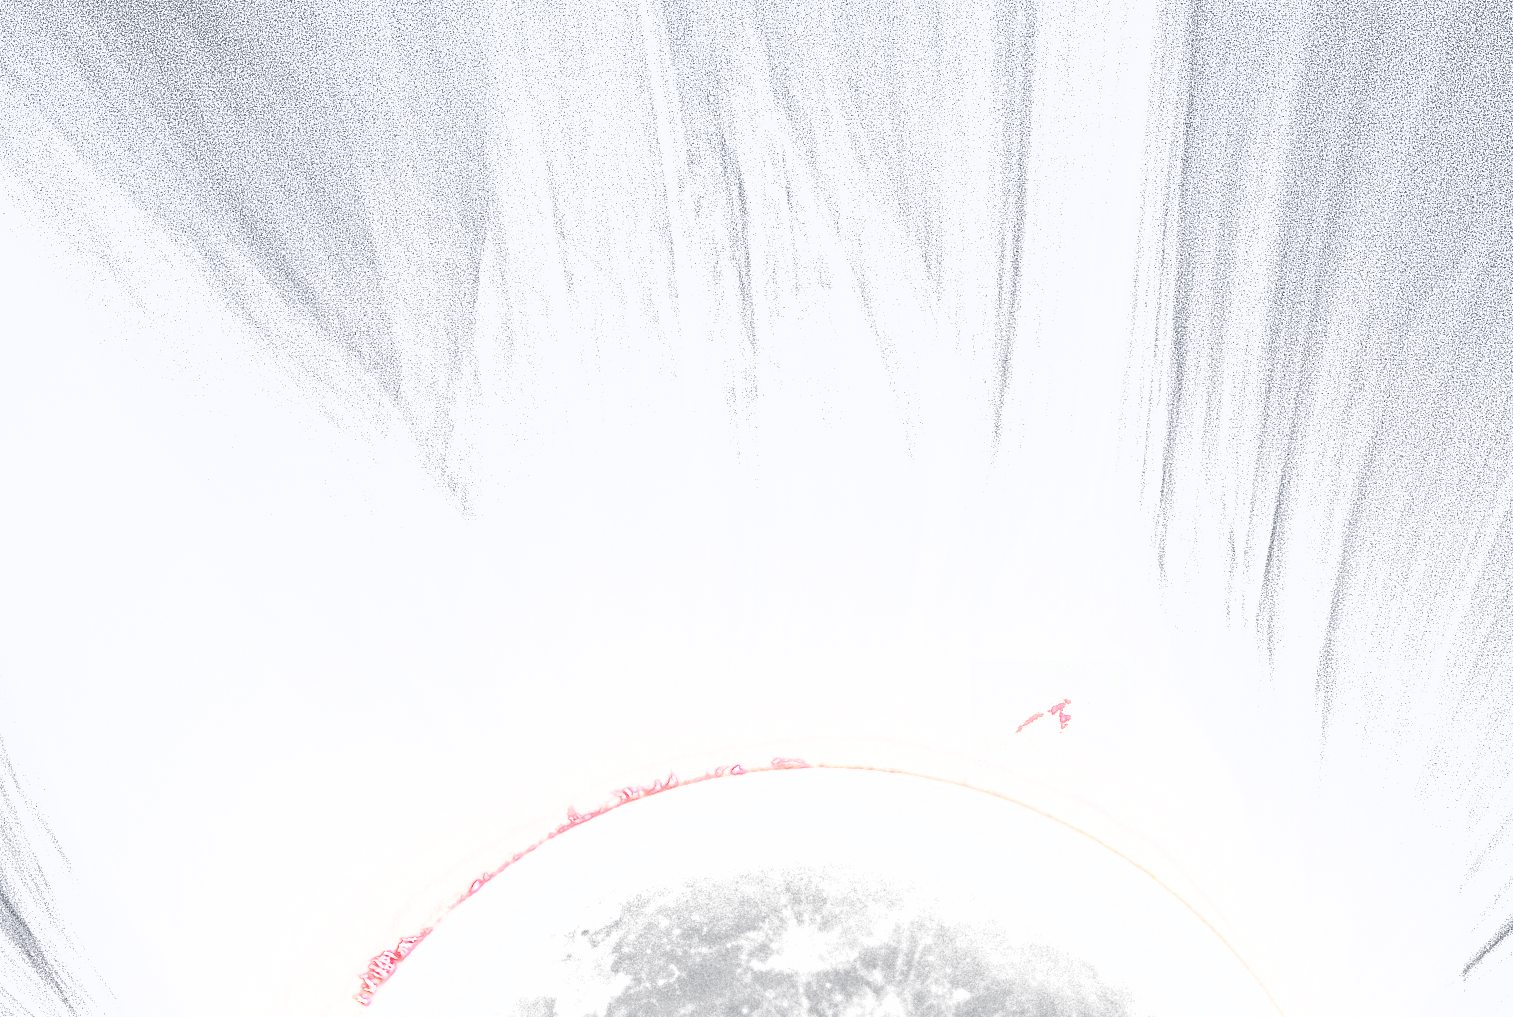
\includegraphics[width=18cm]{titlecorona.png}};
			\fill[Foreground, opacity=0.8] ([yshift=2cm]current page.west) rectangle ([yshift=1cm]current page.east);
			\node[font=\LARGE, Background, anchor=west] at ([yshift=1.5cm, xshift=1cm]current page.west) {\insertsectionhead};
			\node[font=\small, gold, anchor=south west] at ([yshift=2cm]current page.west) {Upcoming:};
		\end{tikzpicture}
	\end{frame}
	}
}

\setbeamertemplate{title page}{%
  \begin{tikzpicture}[remember picture, overlay]
	\fill[red] (current page.north west) rectangle (current page.east);
	\begin{scope}
		\clip (current page.north west) rectangle (current page.east);
		\node[opacity=0.8, anchor=south east, yscale=-1] at ([yshift=2mm, xshift=2cm]current page.north east) {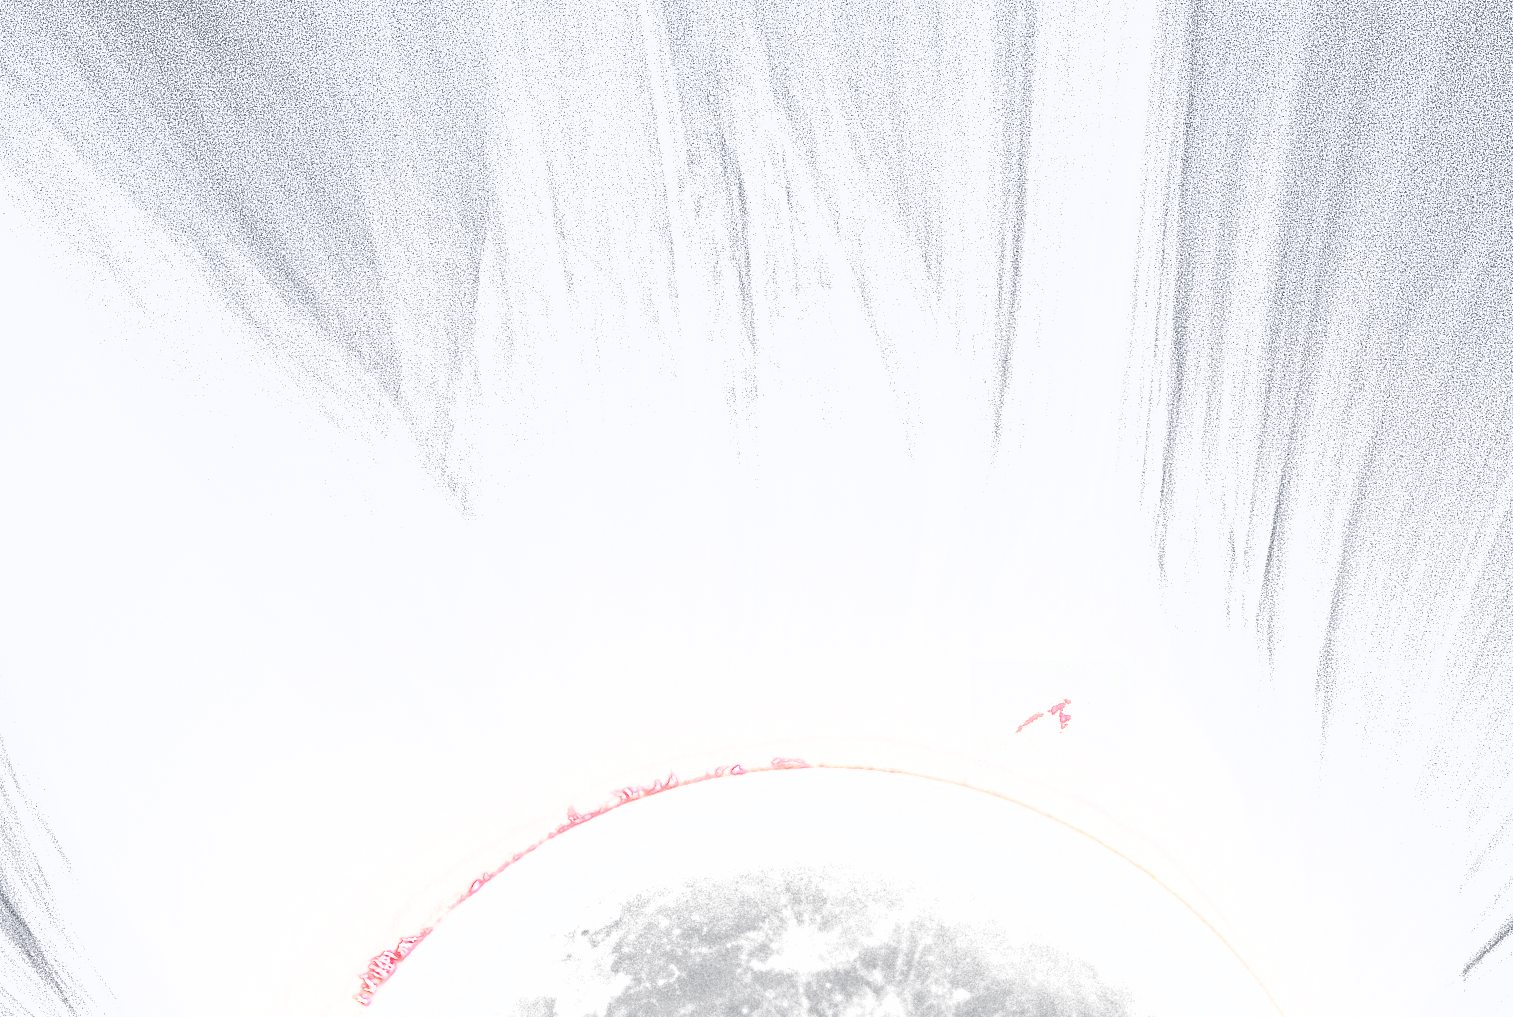
\includegraphics[width=18cm]{titlecorona.png}};
	\end{scope}
	\node[font={\Huge\scshape}, red, anchor=south, inner sep=0pt, outer sep=0pt] at ([yshift=-12mm]current page.center) {\inserttitle};
	\node[font={\Huge\scshape}, black!80, opacity=0.3, anchor=south, inner sep=0pt, outer sep=0pt, yscale=-1, xslant=1.2] at ([yshift=-12mm]current page.center) {\inserttitle};
	\node[font=\large, gold] at ([yshift=-22mm]current page.center) {\insertsubtitle};
	\node[font=\large] (name) at ([yshift=-30mm]current page.center) {\insertauthor};
	\node[gray] at ([yshift=-36mm]current page.center) {\insertinstitute};
  \end{tikzpicture}
}

\newcommand{\credit}[1]{\par\hfill\tiny Credit:~\itshape#1\hspace*{.7cm}}
		

%Preamble
\title{Throwing Shade}
\subtitle{Preparing for the August 21st Eclipse}
\author{Jed Rembold}
\institute{Willamette University}
\date{August 7, 2017}

\begin{document}

{
  \setbeamertemplate{footline}{}
  \maketitle
}

\begin{frame}{Outline}
	\begin{columns}
		\column{0.5\textwidth}
		\begin{itemize}[<+->]
			\item Eclipse Basics
				\begin{itemize}
					\item What are we talking about?
					\item Why are they rare?
					\item Why should we care?
				\end{itemize}
			\item Upcoming eclipse
				\begin{itemize}
					\item How can you observe?
					\item How can you photograph?
					\item Things to look for?
					\item How to survive?
					\item How can you research?!
				\end{itemize}
			\item Closing Remarks
		\end{itemize}	
		\column{0.5\textwidth}
		\begin{figure}[h!]
			\centering
			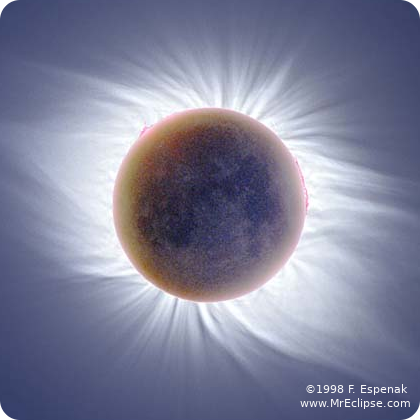
\includegraphics[width=0.8\linewidth]{eclipse1.png}
		\end{figure}
		
	\end{columns}
	
	
\end{frame}

\section{Eclipse Basics}

\begin{frame}{What is an Eclipse?}
	\begin{itemize}
		\item In short, we are talking about a shadow
			\begin{itemize}
				\item Cast by Earth $\Rightarrow$ Lunar Eclipse
				\item Cast by Moon $\Rightarrow$ Solar Eclipse
			\end{itemize}
	\end{itemize}
	\begin{center}
		\only<1>{\includestandalone{Images/ch2_eclipse_moon}}
		\only<2>{\includestandalone{Images/ch2_eclipse_sun}}
		\only<3>{\includestandalone{Images/ch2_eclipse_sun2}}
	\end{center}
\end{frame}

\begin{frame}{But why so uncommon?}
	\begin{columns}
		\column{0.5\textwidth}
		\begin{itemize}[<+->]
			\item Geometry?
				\begin{itemize}
					\item Actually doesn't work
					\item Would see 2 eclipses each month
				\end{itemize}
			\item Need to account for Moon's orbital tilt!
				\begin{itemize}
					\item Leads to only twice a year an eclipse \emph{could} happen
					\item Depends on the lunar phase being just right during that little window
				\end{itemize}
		\end{itemize}	
		\column{0.5\textwidth}
		\begin{center}
			
\includegraphics[width=.7\textwidth]{saros.pdf}\\
			\url{https://goo.gl/Hq6ma1}
		\end{center}
	\end{columns}
\end{frame}

\begin{frame}{Eclipse Geometry}
	\begin{center}
		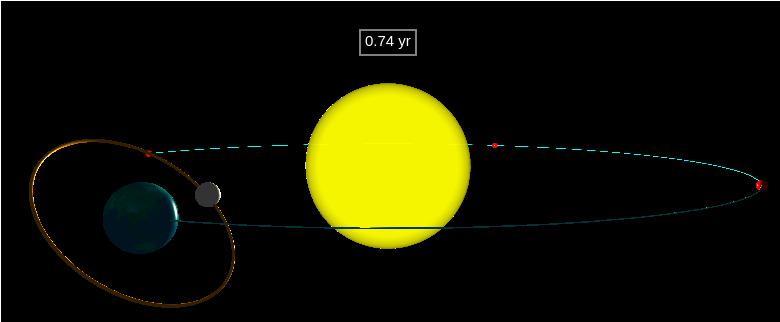
\includegraphics[width=\textwidth]{EclipseGeometry.png}
	\end{center}
\end{frame}

\begin{frame}{Saros Cycle}
	\begin{itemize}
		\item Length of Lunar cycle and length of Earth's orbit give time between Eclipses
		\item Comes out to be about 18 years, 10 days and 8 hours
		\item Fraction of day means the location on Earth moves each cycle
		\item Known as the Saros cycle
			\begin{itemize}
				\item Has been know about since ancient times
			\end{itemize}
			
	\end{itemize}
	\begin{center}
		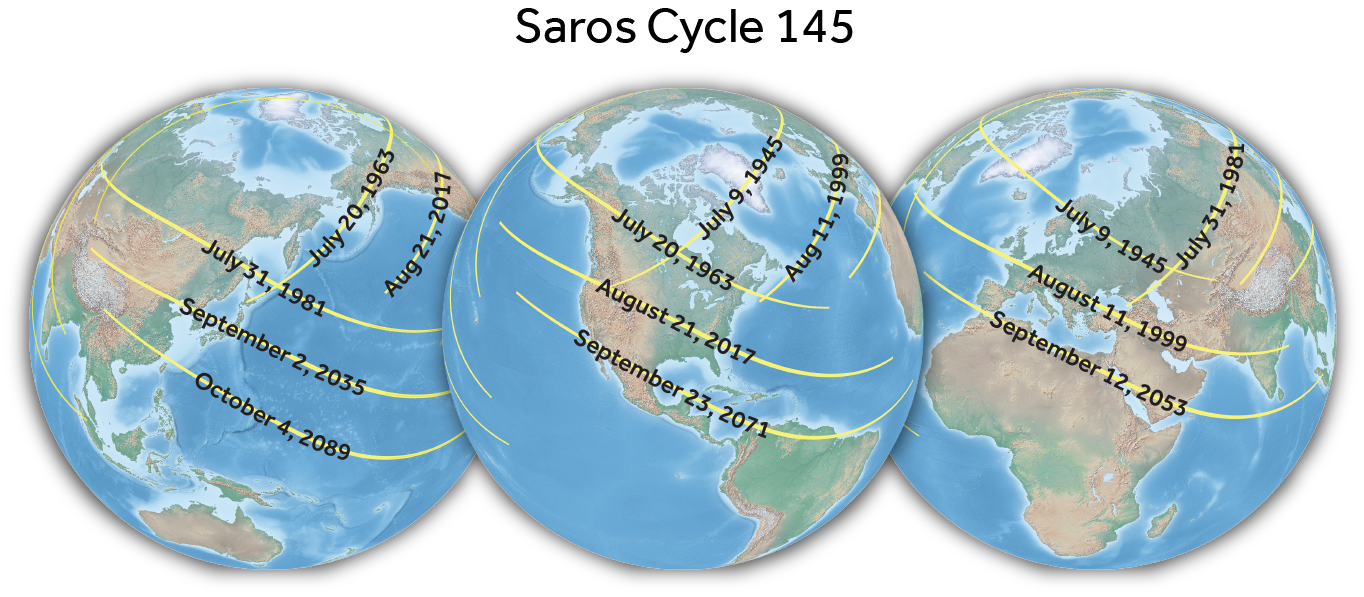
\includegraphics[width=.7\textwidth]{saros.png}
		\credit{www.greatamericansolareclipse.com}
	\end{center}
\end{frame}

\begin{frame}{Why do we care?}
	\begin{itemize}
		\item Likely the most apparent reminder that our planet is part of something greater
		\item Lots of science that can be done!
			\begin{itemize}
				\item Only time the Sun's corona is easily visible
					\begin{itemize}
						\item Information about solar flares, solar wind, and solar weather in general
						\item Affects Earth satellites, astronauts, aurora
					\end{itemize}
				\item Studies of the Earth's atmosphere reacting to solar energy
					\begin{itemize}
						\item Balloons being sent up to measure cooling and heating
						\item Live-streaming footage of the shadow on Earth from the edge of space!
					\end{itemize}
				\item High precision information about lunar terrain
				\item Potential for rare astronomy on stars or planets that tend to be near the Sun and thus invisible
			\end{itemize}
	\end{itemize}
\end{frame}

\section{The Upcoming Eclipse!}
\begin{frame}{The Facts}
	\begin{columns}
		\column{0.5\textwidth}
		\begin{itemize}
			\item<1-> First Contact: 9:05:26am
			\item<2-> Start of Total: 10:17:19am
			\item<2-> Midpoint of Total: 10:18:16am
			\item<2-> End of Total: 10:19:13am
			\item<3-> Last Contact: 11:37:46am
			\item<3-> Duration of Totality: \alert{1 min 54 sec}
		\end{itemize}	
		\column{0.5\textwidth}
		\begin{center}
			\begin{tikzpicture}
				\fill[black] (-3,-3) rectangle (3,3);
				\node[circle, outer color=orange, inner color=yellow, inner sep=0pt, outer sep=0pt, minimum size=2cm] (sun) at (0,0) {};
				\onslide<1>{\node[inner sep=0pt, outer sep=0pt, opacity=0.5] at (45:2) {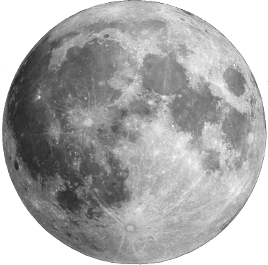
\includegraphics[width=2cm]{ch2_moon_small2.png}};}
				\onslide<2>{
					\node[inner sep=0pt, outer sep=0pt, opacity=0.5] at (45:0) {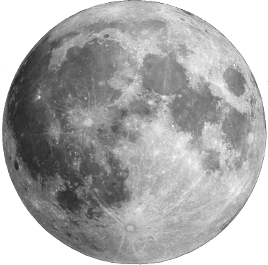
\includegraphics[width=2cm]{ch2_moon_small2.png}};
					\fill[inner color=white, outer color=black, opacity=0.9] (0,0) circle (1.55cm);
					\fill[black, opacity=.9] (0,0) circle (1cm);
				}
				\onslide<3>{\node[inner sep=0pt, outer sep=0pt, opacity=0.5] at (45:-2) {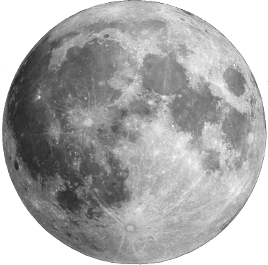
\includegraphics[width=2cm]{ch2_moon_small2.png}};}
			\end{tikzpicture}
		\end{center}
	\end{columns}
\end{frame}

\begin{frame}{Observing Locations}
	Things to keep in mind:
	\begin{itemize}
		\item The sun will be about halfway up in the sky, just South of due East, so make sure you aren't behind a building or tall tree!
		\item Being near water may be good, or it may be bad. I've read some accounts of the cooling causing steam to come up off the water, obscuring things
		\item Scientific demonstrations, experiments and viewing will be happening on the Willamette North Lawn
		\item Plan ahead, and consider walking if possible, because things will probably be \emph{crazy}.
	\end{itemize}
\end{frame}

\begin{frame}{How to Observe}
	\begin{columns}
		\column{0.5\textwidth}
		\begin{itemize}
			\item During totality, you are free to look at the Sun directly without harm
			\item But special viewing equipment needed prior to totality
			\item<2> Let me repeat:
				\begin{alertblock}{Alert!}
					You need special equipment to view the eclipse before or after totality! Sunglasses will not suffice!
				\end{alertblock}
		\end{itemize}	
		\column{0.5\textwidth}
		\begin{center}
			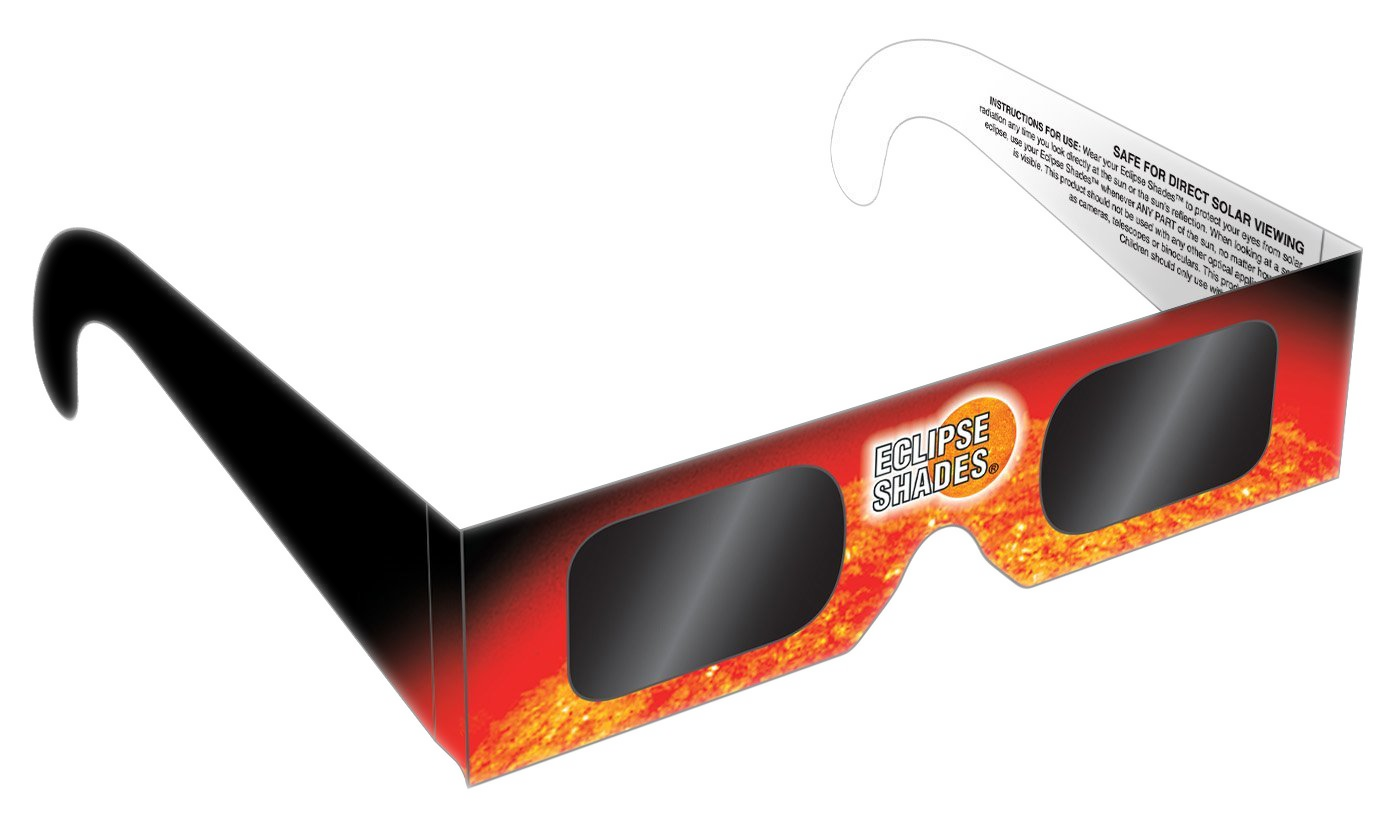
\includegraphics[width=0.8\textwidth]{shades.png}
			\credit{Amazon.com}
		\end{center}
	\end{columns}
\end{frame}

\begin{frame}{Do NOT view using:}
	\begin{center}
		\vspace{-5mm}
		\begin{tikzpicture}
			\onslide<2->{\node[image] at (0,0) {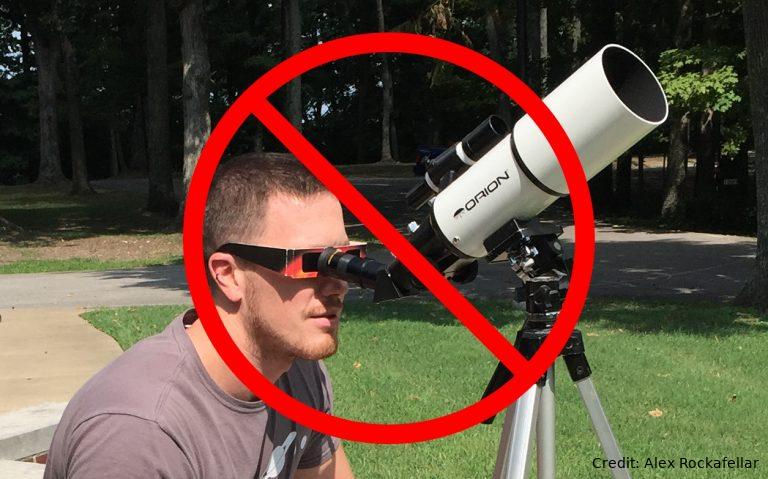
\includegraphics[width=7cm]{dont1.png}};}
			\onslide<3->{\node[image] at (4,2) {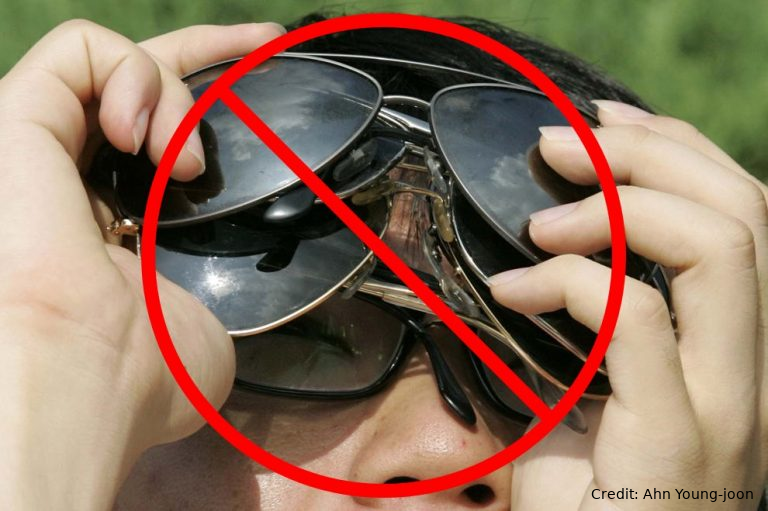
\includegraphics[width=6cm]{dont2.png}};}
			\onslide<4->{\node[image] at (-5,-1) {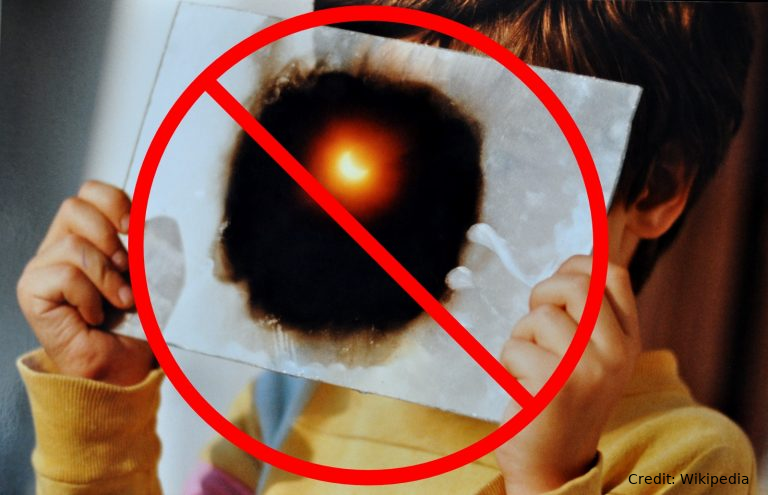
\includegraphics[width=5cm]{dont3.png}};}
			\onslide<5->{\node[image] at (-4,2) {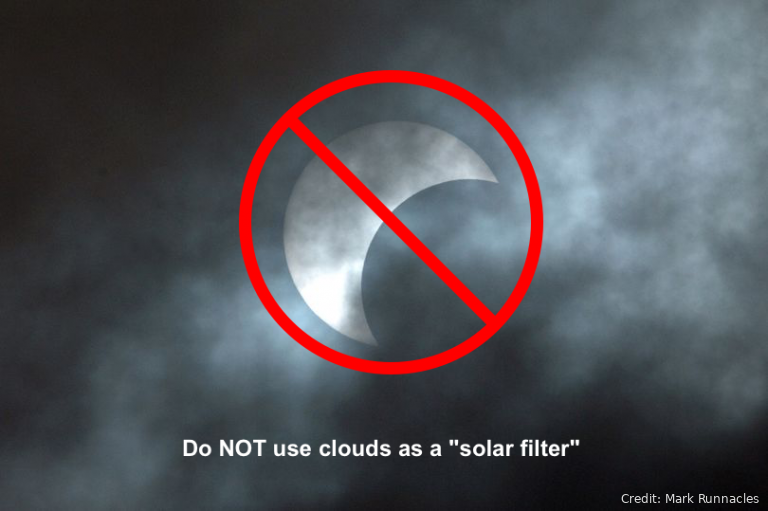
\includegraphics[width=5cm]{dont4.png}};}
			\onslide<6->{\node[image] at (4,-1) {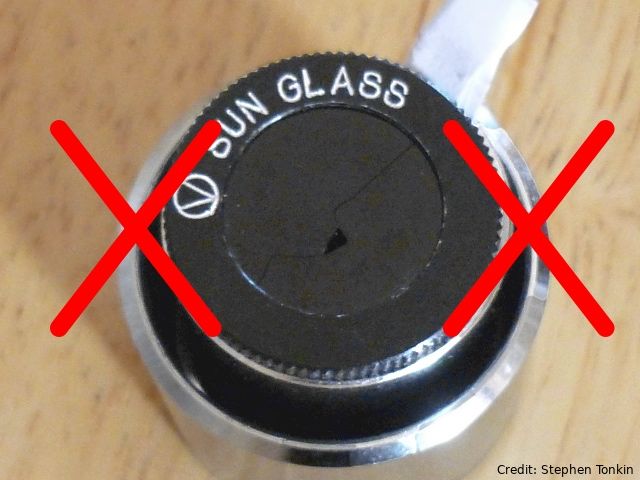
\includegraphics[width=4cm]{dont5.png}};}
		\end{tikzpicture}
		
	\end{center}
\end{frame}


\begin{frame}{DO view using:}
	\begin{itemize}
		\item Solar Eclipse viewing glasses
		\item Welding masks (shade 14 or darker)
		\item Telescopes or binoculars \emph{with solar filters attached}
		\item Pin-hole boxes
		\item Mirror projection
		\item Colander!
	\end{itemize}
	\begin{block}{Rule of Thumb}
		Basically, if you wouldn't want to look at the Sun normally through something, don't look at the eclipse before or after totality with that same something!
	\end{block}
\end{frame}

\begin{frame}{Photography}
	\begin{itemize}
		\item My short recommendation: Don't try too hard
			\begin{itemize}
				\item Getting great eclipse pictures is \emph{tough}
				\item You only have 2 minutes to appreciate a probably once in a lifetime event
				\item Spend a second or two snapping a shot if you want, but then just observe everything around you!
			\end{itemize}
		\item If you do want to try your luck though:
			\begin{itemize}
				\item Shots before or after totality need the same protection as your eyeballs!
				\item \alert{Do not use any flash!}
				\item You'll want a tripod
				\item You'll likely want at least a \SI{300}{\milli\meter} focal length lens for the Sun to be a decent size in the field of view
				\item Focus on the Moon in the nights beforehand and tape down the focus position
				\item Make sure everything is covered and protected again before totality finishes
			\end{itemize}
	\end{itemize}
\end{frame}

\begin{frame}{Some Things to Look For}
	\begin{columns}
		\column{0.5\textwidth}
		\begin{center}
			\includegraphics<1>[width=0.8\textwidth]{treeeffect.png}
			\only<1>{\credit{Ed Morana}}
			\includegraphics<2>[width=0.8\textwidth]{firstcontact.jpg}
			\only<2>{\credit{Mitzi Adams}}
			\includegraphics<3>[width=0.8\textwidth]{diamondring.jpg}
			\only<3>{\credit{Pedro R\'e}}
			\includegraphics<4>[width=0.8\textwidth]{bailysbeads.jpg}
			\only<4>{\credit{Ragnar Axelsson}}
			\includegraphics<5>[width=0.8\textwidth]{corona.jpg}
			\only<5>{\credit{NASA Goddard Space Flight Center}}
			\includegraphics<6>[width=0.8\textwidth]{sky.png}
			\only<6>{\credit{Billy Teets}}
		\end{center}
		\column{0.5\textwidth}
		\begin{itemize}
			\item<1-> Tree pinhole cameras!
			\item<2-> First and Last Contact
			\item<3-> The Diamond Ring
			\item<4-> Baily's Beads
			\item<5-> The Solar Corona
			\item<6-> Planets!
		\end{itemize}
	\end{columns}
\end{frame}

\begin{frame}{Effects of the Eclipse}
	\begin{itemize}
		\item Slight lowering of local temperatures (thank goodness...)
			\begin{itemize}
				\item Can lead to an odd "eclipse wind" or breeze
			\end{itemize}
		\item Animals tend to assume nightfall and adopt that behavior
			\begin{itemize}
				\item Birds quiet, wildlife head towards nightly resting grounds, etc
				\item The return of the sun 2 minutes later can leave animals in some confusion and apprehension
			\end{itemize}
		\item People's responses vary. Speechless, screaming, fear, goosebumps, and a sense of sharing in the moment have all been used to describe reactions.
	\end{itemize}
\end{frame}

\begin{frame}{Descriptions}
	\begin{quote}
		An assembled crowd is awed into silence almost invariably. Trivial chatter and senseless joking cease. Sometimes the shadow engulfs the observer smoothly, sometimes apparently with jerks; but all the world might well be dead and cold and turned to ashes. Often the very air seems to hold its breath for sympathy; at other times a lull suddenly awakens into a strange wind, blowing with unnatural effect.

		Then out upon the darkness, gruesome but sublime, flashes the glory of the incomparable corona, a silvery, soft, unearthly light, with radiant streamers, stretching at times millions of uncomprehended miles into space, while the rosy, flame-like prominences skirt the black rim of the moon in ethereal splendor.
		\begin{flushright}
			Mabel Loomis Todd - Total Eclipses of the Sun, 1894
		\end{flushright}
	\end{quote}
\end{frame}

\begin{frame}{How to Survive!}
	\begin{center}
		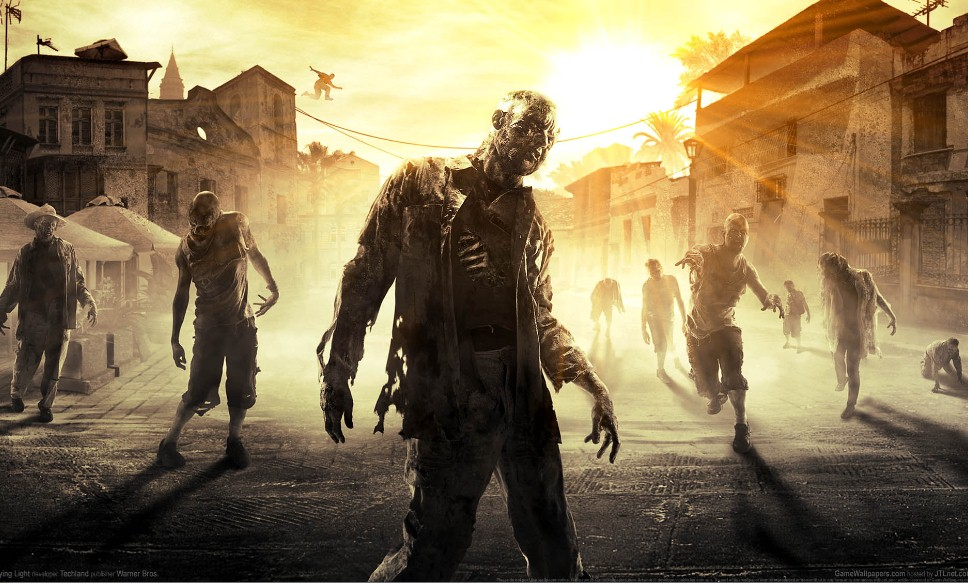
\includegraphics[width=0.8\textwidth]{zombie.jpg}
		\credit{breakoutfortmc.com}
	\end{center}
\end{frame}

\begin{frame}{Recommendations}
	\begin{itemize}
		\item Estimates are for a million people 
			\begin{itemize}
				\item Oregon normally has a population of 4 million
				\item Most will be coming here to Salem or Madras
			\end{itemize}
		\item Traffic is likely to be horrible if moving at all. Prepare accordingly
		\item Don't do anything dumb. Paramedics, fire departs, etc will be overworked and similarly encumbered
		\item You may want to make any grocery runs before the weekend of the eclipse
		\item Cell phone networks may be stressed
		\item Basically, prepare. It is going to be quite a thing. Think of it as a mild dry run for your disaster planning...
	\end{itemize}
\end{frame}

\begin{frame}{Help Science!}
	\begin{itemize}
		\item Check out the work being done on the North Lawn of Willamette, but be respectful of the work people are doing
		\item Understand that for many eclipse scientists, the event is rather stressful with all the data they need to try to collect in a very small time frame!
		\item Want to get involved yourself? Check out the GLOBE Observer app on your phone:
			\begin{center}
				\url{https://observer.globe.gov/about/get-the-app}
			\end{center}
			\begin{itemize}
				\item Solar Eclipse portion to be released on August 18
				\item Mainly interested in cloud observations or temperature observations in the hours before and after the eclipse.
			\end{itemize}
	\end{itemize}
\end{frame}

\begin{frame}{Have Fun!}
	\begin{itemize}
		\item Plan ahead
			\begin{itemize}
				\item You will probably be less stressed if you don't drive anywhere
				\item Ensure you'll have a view to the East without trees, buildings, or street lights
			\end{itemize}
		\item Make sure you have proper viewing equipment
		\item Don't get caught up in trying to take the perfect picture
		\item Take a moment to look down during totality to observe everyone around you
		\item Make it memorable! (safely!)
	\end{itemize}
\end{frame}

\begin{frame}{Questions?}
	\begin{itemize}
		\item Links
			\begin{itemize}
				\item Tilt Simulation: \url{https://goo.gl/Hq6ma1}
				\item NASA Streams: \url{https://eclipse2017.nasa.gov/eclipse-live-stream}
				\item Balloon Stream: \url{http://eclipse.stream.live/}
			\end{itemize}
			
	\end{itemize}
	
\end{frame}

















\end{document}

